\documentclass[a4paper,10pt]{article}

\usepackage{fullpage}
\usepackage{graphicx}
\usepackage{amsmath}
\usepackage{amssymb}

% Title Page
\title{Baby Brain Toolkit}
\author{Fbrain ERC project: Computational Anatomy of Fetal Brain}


\begin{document}
\maketitle
\tableofcontents
%\begin{abstract}
%\end{abstract}

\section{Introduction}

BTK stands for Baby Brain Toolkit. This toolkit is developed in the context of
the Fbrain ERC project: ``Computational Anatomy of Fetal
Brain''\footnote{http://lsiit-miv.u-strasbg.fr/miv/index.php?contenu=erc}. 
Studies about brain maturation aim at providing a better understanding of brain
development and links between brain changes and cognitive development. Such
studies are of great interest for diagnosis help and clinical course of
development and treatment of illnesses. Several teams have begun to make 3D maps
of developing brain structures from children to young adults. However, working
out the development of fetal and neonatal brain remains an open issue. This
project aims at jumping over several theoretical and practical barriers and at
going beyond the formal description of the brain maturation thanks to the
development of a realistic numerical model of brain aging.

\subsection{Copyright}
This software is governed by the CeCILL-B license under French law and
abiding by the rules of distribution of free software.  You can  use, 
modify and/ or redistribute the software under the terms of the CeCILL-B
license as circulated by CEA, CNRS and INRIA at the following URL
"http://www.cecill.info". 

As a counterpart to the access to the source code and rights to copy,
modify and redistribute granted by the license, users are provided only
with a limited warranty  and the software's author,  the holder of the
economic rights,  and the successive licensors  have only  limited
liability. 

In this respect, the user's attention is drawn to the risks associated
with loading,  using,  modifying and/or developing or reproducing the
software by the user in light of its specific status of free software,
that may mean  that it is complicated to manipulate,  and  that  also
therefore means  that it is reserved for developers  and  experienced
professionals having in-depth computer knowledge. Users are therefore
encouraged to load and test the software's suitability as regards their
requirements in conditions enabling the security of their systems and/or 
data to be ensured and,  more generally, to use and operate it in the 
same conditions as regards security. 

\subsection{Installation}

\subsubsection{Dependencies}

Baby Brain Toolkit (BTK) needs the following packages:
\begin{itemize}
 \item CMake (www.cmake.org), Tclap (tclap.sourceforge.net), OpenMP (openmp.org), VTK (www.vtk.org), ANN (www.cs.umd.edu/\string~mount/ANN). These libraries can be installed using the following command line: 
 \begin{itemize}
 \item for debian-based distributions: \texttt{apt-get install cmake cmake-curses-gui libtclap-dev libgomp1 libvtk5-dev libann-dev}
 \item for MacOSX using macports: \texttt{port install cmake tclap vtk5 libANN}
 \end{itemize}
 \item Install Git: this library can be installed using the following command line : 
 \begin{itemize}
 \item for debian-based distribution: \texttt{apt-get install git-core}
 \item for MacOSX using macports: \texttt{port install git-core}
 \end{itemize}
 \item Insight Toolkit (ITK) version 4:
\begin{verbatim}
git clone git://itk.org/ITK.git
mkdir ITK-build
cd ITK-build
ccmake ../ITK/
\end{verbatim}
This will bring up the CMake configuration screen. Press \texttt{[c]} for configure and then use \texttt{[t]} to toggle the advanced mode. Make the following changes:
\begin{verbatim}
BUILD_TESTING = OFF
CMAKE_BUILD_TYPE = Release
ITK_USE_REVIEW = ON
ITK_BUILD_ALL_MODULES = ON
\end{verbatim}
Then press \texttt{[c]} to configure and \texttt{[g]} to generate the make file. Finally, type \texttt{make} at the prompt to obtain the final build of ITK.

\end{itemize}

\subsubsection{Download and compile the BTK sources}
\begin{itemize}
 \item Get the BTK sources: \texttt{git clone https://github.com/rousseau/fbrain.git }
 \item Then:
\begin{verbatim}
mkdir fbrain-build
cd fbrain-build
ccmake ../fbrain
make
\end{verbatim}
\end{itemize}

Most of the programs of the BTK suite use the OpenMP library for multi-threading
purpose. The number of cores used can be tuned using the following command line
(in this example, 4 cores will be used): \texttt{export OMP\_NUM\_THREADS=4}
\section{The whole pipeline}
BTK allows to implement the whole pipeline for the processing of fetal images,
i.e. the reconstruction of anatomical and diffusion data, and the final
tractography, all expressed in the same local coordinate system. This
processing can be summarized in the following steps:

\begin{enumerate}
 \item Image conversion
 \item Anatomical image reconstruction
 \item Recontruction of the diffusion sequence
 \item Registration of diffusion to anatomical data
 \item Tractography
\end{enumerate}

In the following we explain the applications and utilities to use for each of
the aforementioned steps.

\subsection{Image conversion}
BTK supports and has been tested by using images in Nifti format
(http://nifti.nimh.nih.gov/nifti-1). However, images are frequently available in
DICOM format and an image conversion is required. This can be performed by using
dcm2nii, a converter freely available at http://www.cabiatl.com/mricro/mricron/
dcm2nii.html. In this site you can find other options that can be best suited
for your data.

\subsection{Anatomical image reconstruction}
This can be performed by using \textbf{btkImageReconstruction} (Section
\ref{subsec:ana_rec}) followed by \textbf{btkReorientImageToStandard} (Section
\ref{sec:utilities}) to transform the result to a standard orientation.

\subsection{Reconstruction of the diffusion sequence}
To reconstruct diffusion data, you want to follow the steps described in
Section \ref{subsec:diff_rec}. The use of two applications is required here:
\textbf{btkGroupwiseS2SDistortionCorrection} and
\textbf{btkRBFInterpolationS2S}.

\subsection{Registration of diffusion to anatomical data}
TO BE WRITTEN

\subsection{Tractography}
If you have followed the previous steps correctly, at this point you should
have the reconstructed anatomical and diffusion data spatially aligned, and
ready to perform the tractography. To do this, BTK provides
\textbf{btkTractography} (Section \ref{subsec:tracto})

\section{Applications}

\subsection{Denoising}

\begin{description}
 \item[btkNLMDenoising] This program applies a non-local mean filter to a 3D image for denoising purpose. Usage: \texttt{-i input\_image\_filename -o output\_image\_filename}. The best results are usually obtained by using a mask (or a padding value).
\end{description}

\begin{description}
 \item[btkNLMDenoising4DImage] This program applies a non-local mean filter to each 3D image of a 4D image, for denoising purpose. Usage: \texttt{-i input\_image\_filename -o output\_image\_filename}. The best results are usually obtained by using a mask (or a padding value).
\end{description}


\subsection{Anatomical reconstruction}

\begin{description}
 \item[btkImageReconstruction] This program allows to obtain a
high-resolution image from a set of low-resolution images, typically
axial, coronal, and sagital acquisitions~\cite{Rousseau2006}. \\\\
Minimal usage: \texttt{btkImageReconstruction -i image1 $\cdots$ -i imageN -o
output}. 

Recommended usage: \texttt{btkImageReconstruction -i image1 $\cdots$ -i imageN
-m mask1 $\cdots$ -m maskN -o output --mask}. The use of a mask provide
better results since it allows an accuratelly estimation of the initial
transform, and constrains the registration to the region of interest.

The full list of optional parameters of the method can be obtained by
\texttt{btkImageReconstruction --help}

\end{description}

\begin{figure}[t]
\centering
\begin{tabular}{ccc}
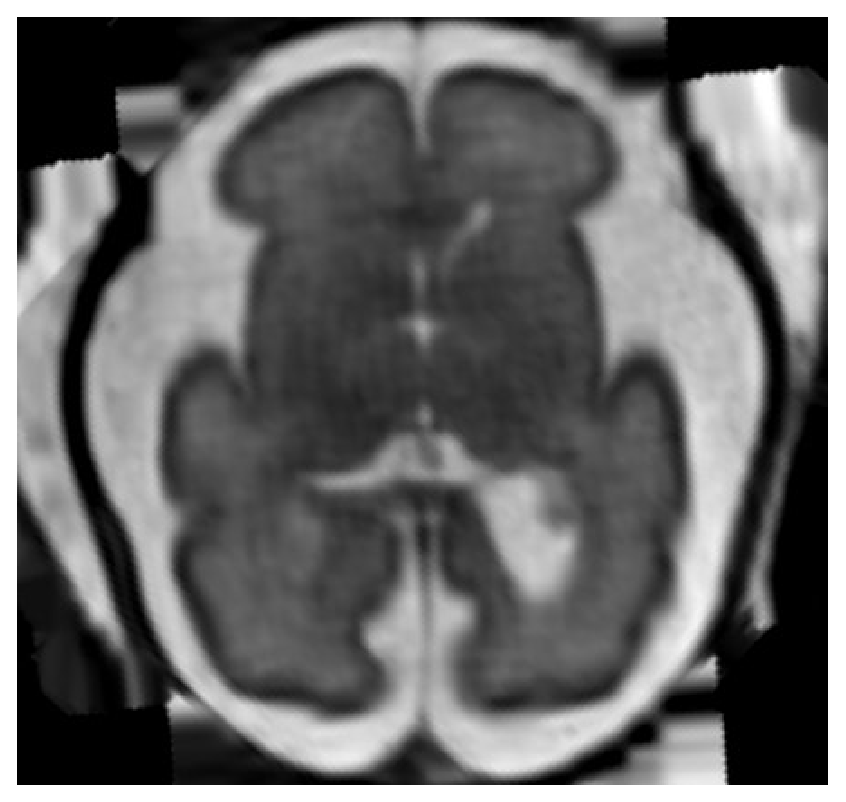
\includegraphics[width=0.3\columnwidth]{hr_axl.eps}&
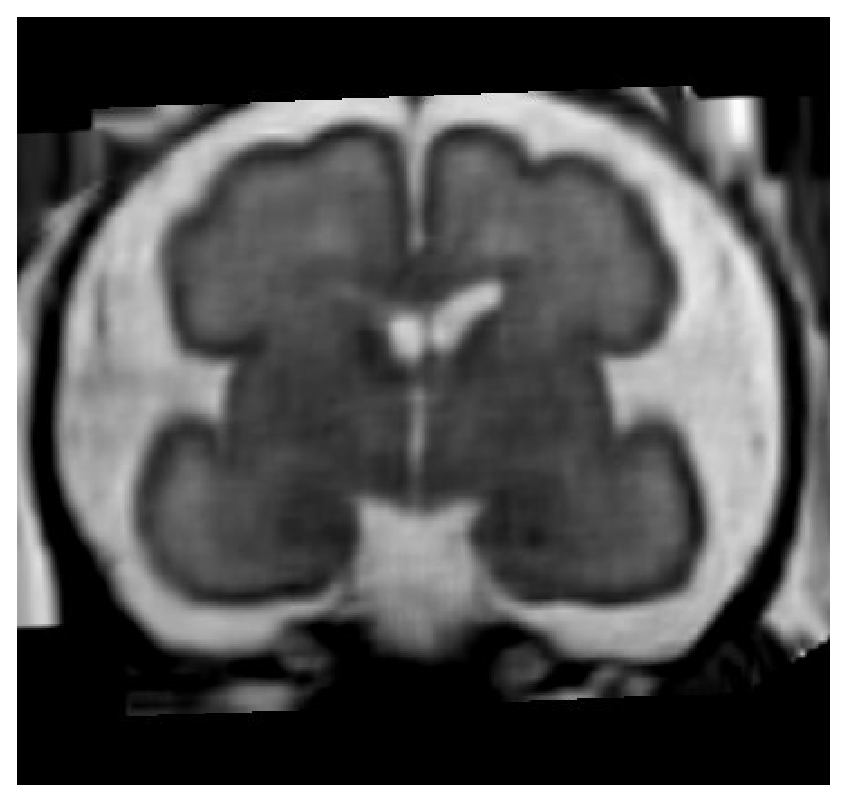
\includegraphics[width=0.3\columnwidth]{hr_cor.eps}&
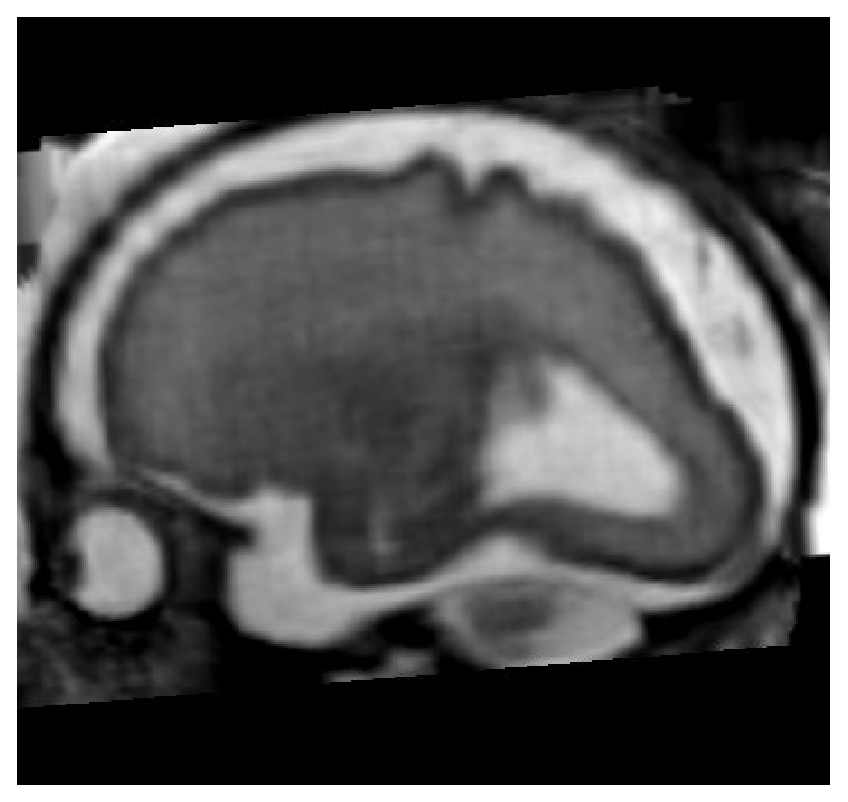
\includegraphics[width=0.3\columnwidth]{hr_sag.eps}\\
{(a)}&{(b)}&{(c)}\\
\end{tabular}
\caption{Example of an anatomical reconstruction of a fetal brain by using
\texttt{btkImageReconstruction}. (a) axial, (b) coronal, and (c) sagital view.}
\label{fig:reconstruction}
\end{figure}


\subsection{Tractography}

\begin{description}
 \item[btkTractography] This program performs a probabilistic tractography using a particle filtering. Usage: \texttt{-d dwi\_image\_filename -v dwi\_gradient\_vectors -m white\_matter\_mask -l seeds\_la\-bel\_image}.
\end{description}

\newpage
\section{Utilities}
\label{sec:utilities}


\addcontentsline{toc}{subsection}{btkApplyMaskToImage}
\addcontentsline{toc}{subsection}{btkAverage3DImages}
\addcontentsline{toc}{subsection}{btkAverageImagesWithReference}
\addcontentsline{toc}{subsection}{btkBinarizeLabels}
\addcontentsline{toc}{subsection}{btkBinarizeTissueProbabilityMaps}
\addcontentsline{toc}{subsection}{btkComputeChamferDistance}
\addcontentsline{toc}{subsection}{btkComputeOverlap}
\addcontentsline{toc}{subsection}{btkConvertGradientTable}
\addcontentsline{toc}{subsection}{btkCropImageUsingMask}
\addcontentsline{toc}{subsection}{btkDifferentialBiasCorrection}
\addcontentsline{toc}{subsection}{btkExtractOneImageFromSequence}
\addcontentsline{toc}{subsection}{btkFCMClassification}
\addcontentsline{toc}{subsection}{btkImageGaussianFilter}
\addcontentsline{toc}{subsection}{btkImageInjection}
\addcontentsline{toc}{subsection}{btkImageMorphologicalClosing}
\addcontentsline{toc}{subsection}{btkImageMorphologicalTopHat}
\addcontentsline{toc}{subsection}{btkImageResampling}
\addcontentsline{toc}{subsection}{btkImageSimilarity}
\addcontentsline{toc}{subsection}{btkImageSubtract}
\addcontentsline{toc}{subsection}{btkIteratedBackProjection}
\addcontentsline{toc}{subsection}{btkMajorityVoting}
\addcontentsline{toc}{subsection}{btkMidwayHistogramEqualization}
\addcontentsline{toc}{subsection}{btkModifyImageUsingLookUpTable}
\addcontentsline{toc}{subsection}{btkNiftiToNrrd}
\addcontentsline{toc}{subsection}{btkNrrdToNifti}
\addcontentsline{toc}{subsection}{btkPSNR}
\addcontentsline{toc}{subsection}{btkPrintImageInfo}
\addcontentsline{toc}{subsection}{btkProbabilityMapNormalization}
\addcontentsline{toc}{subsection}{btkReconstructionComparisonTool}
\addcontentsline{toc}{subsection}{btkRegisterDiffusionToAnatomicalData}
\addcontentsline{toc}{subsection}{btkReorientDiffusionSequenceToStandard}
\addcontentsline{toc}{subsection}{btkReorientImageToStandard}
\addcontentsline{toc}{subsection}{btkResampleLabelsByInjection}
\addcontentsline{toc}{subsection}{btkRescaleIntensity}
\addcontentsline{toc}{subsection}{btkSequenceNormalization}
\addcontentsline{toc}{subsection}{btkSetStandardCoorSystem}
\addcontentsline{toc}{subsection}{btkSimulateMotionSliceBySlice}
\addcontentsline{toc}{subsection}{btkSimulateStandardViewFromIsotropicImage}
\addcontentsline{toc}{subsection}{btkWarpTransformationToImage}
\addcontentsline{toc}{subsection}{btkWeightedMean}


\begin{description}

\item[btkModifyImageUsingLookUpTable] This program modifies one image using a
look up table defined in a ascii file (2 columns, one for the original values,
one for the final values). Usage: \texttt{-i input\_image\_filename -t
input\_table\_filename -o output\_image\_filename}
  
\item[btkExtractOneImageFromSequence] This program extracts one image from a 4D sequence. Usage: \texttt{-i input\_image\_filename -o output\_image\_filename --image\_index index}

\item[btkNrrdToNifti] This program convert an image from Nrrd file (*.nhdr and *.nrrd) to a Nifti file (*.nii or *.nii.gz). The conversion of a DWI image is possible by using the option \texttt{--dwi}. Usage: \texttt{-i input.nhdr -o output.nii.gz}. Usage for DWI sequence: \texttt{--dwi -i input.nhdr -o output.nii.gz}.

\item[btkNiftiToNrrd] This program convert a diffusion sequence in nifti
format\footnote{Currently there is no nifti standard for DWI, so DW images are
saved as a standard nifti sequence (*.nii, *.nii.gz) and two text files
containing the b-values (.bval) and the gradient directions (.bvec).}  to the
nrrd format (*.nhdr). 

Usage: \texttt{-i input -o output.nhdr}

The list of optional parameters can be obtained by \texttt{btkNiftiToNrrd
--help}

\item[btkReorientImageToStandard] Sometimes it is useful
to reorient the image to the standard orientation. This is necessary with fetal
images since in general the fetus is in a random orientation with respect to the
scanner.

Usage: \texttt{btkReorientImageToStandard -i image -o output -l landmarks}.
\texttt{landmarks} is a text file containing points that define the left-right
and the posterior-anterior directions. The points $l$ and $r$ define the left
$\rightarrow$ right direction, and the points $p$ and $a$ define the posterior
$\rightarrow$ anterior direction. Such file can be easily generated by using
Slicer\footnote{http://www.slicer.org} as follows:

\begin{enumerate}
\item Open the high-resolution image by using the \textit{Volume} module.
\item Toogle on the visibility of all slices in the 3D view. This allows to
identify the left and right sides of the brain in the 2D views.
\item Place the landmarks $l$, $r$, $p$, and $a$ in this order by using
\texttt{[p]}.
\item Save the file (*.fcsv) by using the menu File $\rightarrow$ Save.
\end{enumerate}


\begin{figure}[t]
\centering
\begin{tabular}{ccc}
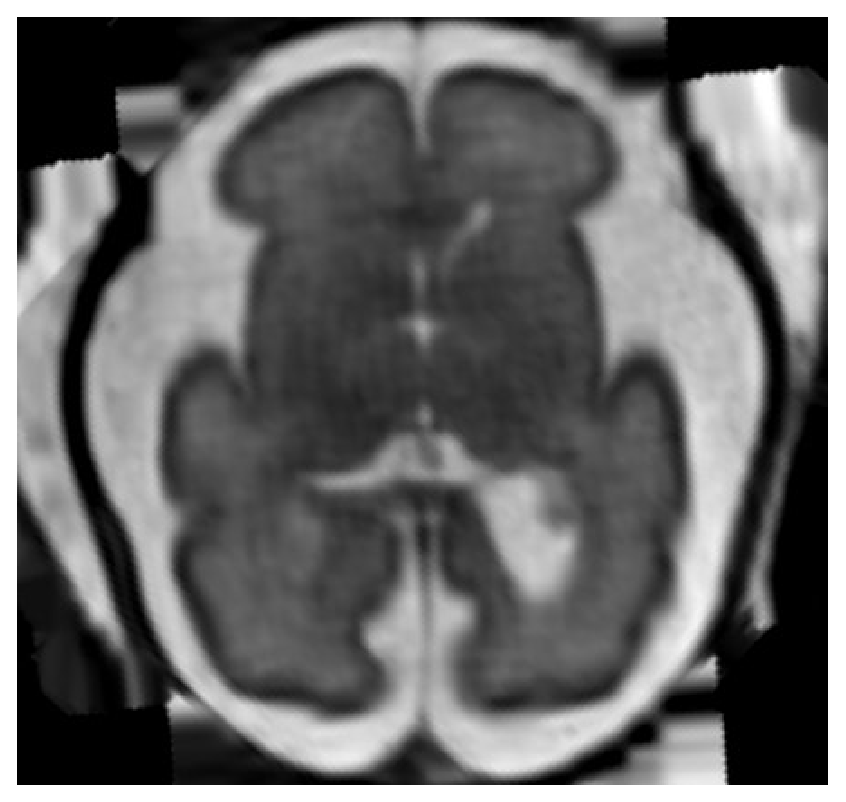
\includegraphics[width=0.3\columnwidth]{hr_axl.eps}&
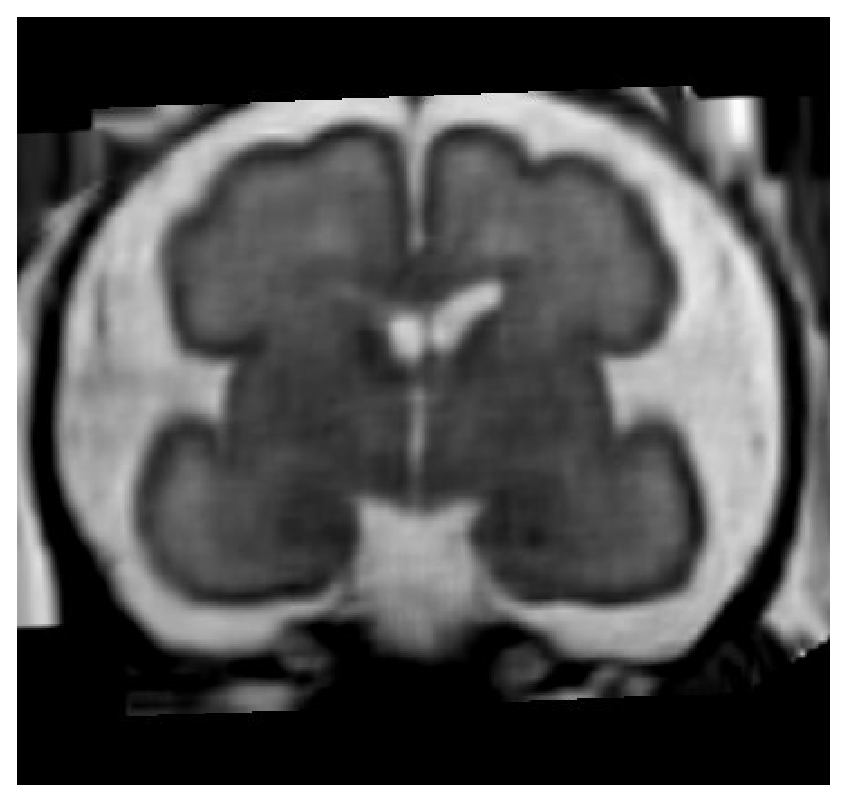
\includegraphics[width=0.3\columnwidth]{hr_cor.eps}&
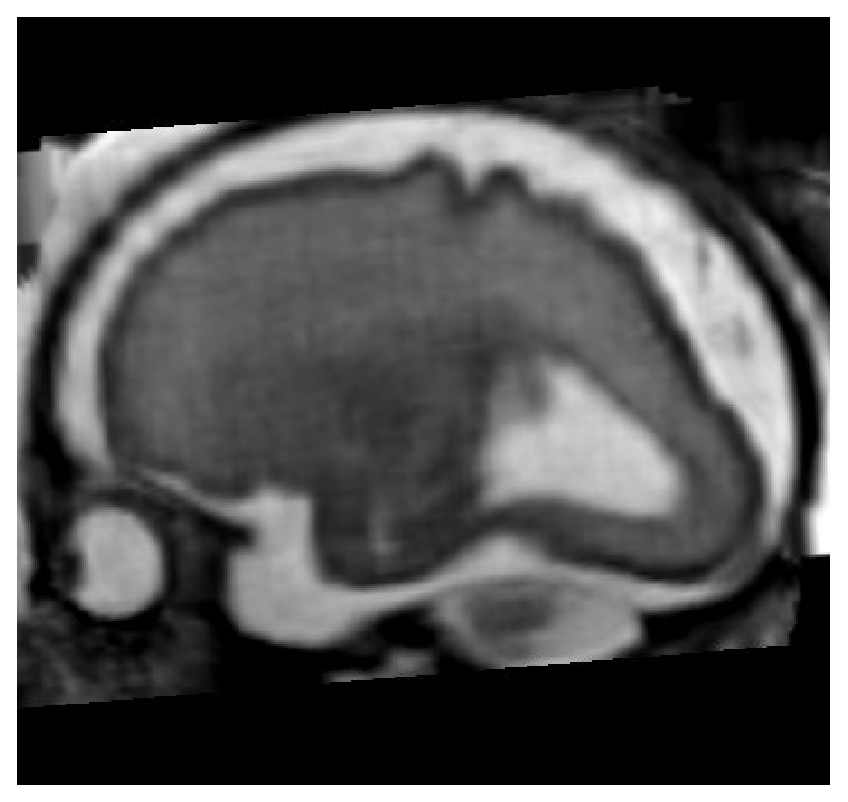
\includegraphics[width=0.3\columnwidth]{hr_sag.eps}\\
{(a)}&{(b)}&{(c)}\\
\end{tabular}
\caption{Example of an anatomical reconstruction of a fetal brain by using
\texttt{btkImageReconstruction}. (a) axial, (b) coronal, and (c) sagital view.}
\label{fig:reconstruction}
\end{figure}

\begin{figure}[t]
\centering
\begin{tabular}{cc}
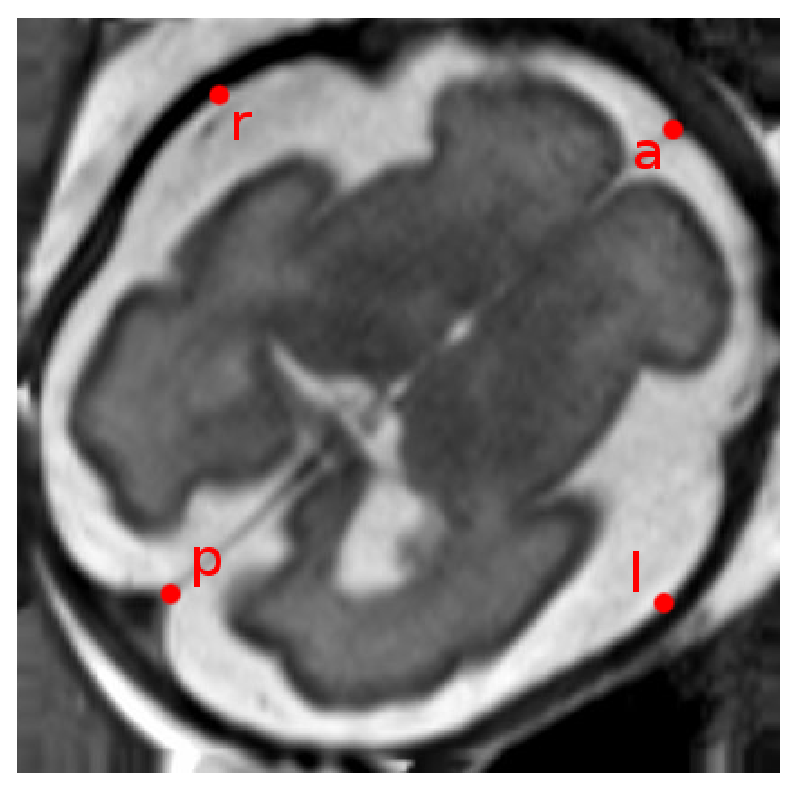
\includegraphics[width=0.35\columnwidth]{lmks_axial.eps}&
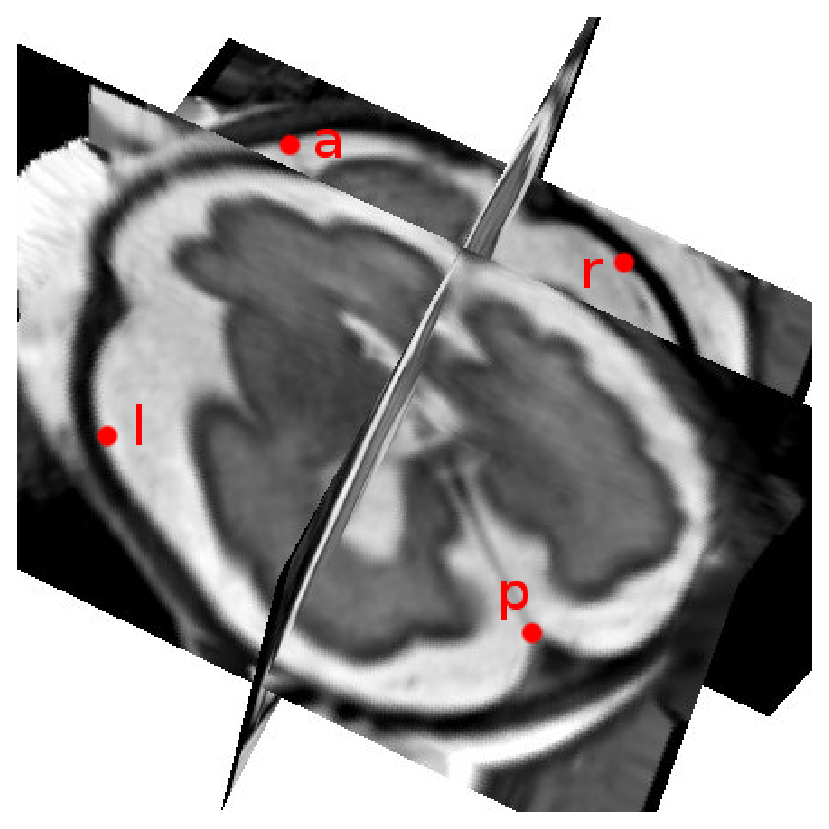
\includegraphics[width=0.35\columnwidth]{lmks_3D.eps}\\
{(a)}&{(b)}\\
\end{tabular}
\caption{Placement of landmarks by using Slicer. (a) axial slice, (b) 3D view.}
\label{fig:landmarks}
\end{figure}

  \item[btkReorientDiffusionSequenceToStandard] Reorients a DW sequence
to the standard orientation. This is necessary with fetal images since the fetus
is in a random orientation with respect to the scanner. This is particularly
important in DWI because colormaps lack of significance, which makes difficult
the identification of specific bundles 

Usage: \texttt{btkReorientDiffusionSequenceToStandard -i image -o output -l
landmarks}.

\texttt{landmarks} is a landmarks file obtained as explained above.

\item[btkCropImageUsingMask] This program crops one (3D or 4D) image using a 3D mask. Usage: \texttt{-i input\_image\_filename -m
input\_mask\_filename -o output\_image\_filename -d 3}, where '-d' is the dimension of the input image (by default 3).

\item[btkRegisterDiffusionToAnatomicalData] This program registers a DW
sequence to an anatomical image. 

Recommended usage: \texttt{btkReorientDiffusionSequenceToStandard -i input
-o output -r reference.nii --mask mask.nii}.
\begin{itemize}
\item[-i] input sequence
\item[-o] resampled sequence (by default, linear interpolation is used)
\item[-r] reference image (anatomical image)
\item[-m] image mask for the B0 image
\end{itemize}

The list of optional parameters can be obtained by \texttt{btkNiftiToNrrd
--help}

\item[btkImageInjection] This program performs the injection of a set
of images with an already existing set of transformations. This avoids the need
to perform a new image reconstruction (computationally expensive) after
modification of the input images (some filtering for example) or an involuntary
deletion of the reconstructed image.

Recommended usage: \texttt{btkImageInjection -i image1 $\cdots$ -i
imageN -m mask1 $\cdots$ -m maskN -t transform1 $\cdots$ -t
transformN -o output --mask}.
\begin{itemize}
\item[-i] input image
\item[-m] image mask
\item[-t] image transform
\item[-o] reconstructed image
\end{itemize}

The list of optional parameters can be obtained by \texttt{btkImageInjection
--help}

\end{description}


\section*{Acknowledgment}
\small{The research leading to these results has received funding from the
European Research Council under the European Community’s Seventh Framework
Programme (FP7/2007-2013 Grant Agreement no. 207667).}

\bibliographystyle{plain}
\bibliography{btk.bib}

\end{document}
